\section{寄存器描述}
\regover{
{\hyperref[gpip-gpadc-config]{gpadc\_config}}&GPADC configuration
\\
\hline
{\hyperref[gpip-gpadc-dma-rdata]{gpadc\_dma\_rdata}}&GPADC DMA read data
\\
\hline
{\hyperref[gpip-gpdac-config]{gpdac\_config}}&GPDAC configuration
\\
\hline
{\hyperref[gpip-gpdac-dma-config]{gpdac\_dma\_config}}&GPDAC dma configuration
\\
\hline
{\hyperref[gpip-gpdac-dma-wdata]{gpdac\_dma\_wdata}}&GPDAC dma write data
\\
\hline
{\hyperref[glb-gpdac-ctrl]{gpdac\_ctrl}}&GPDAC control
\\
\hline
{\hyperref[glb-gpdac-actrl]{gpdac\_actrl}}&GPDAC channelA control
\\
\hline
{\hyperref[glb-gpdac-bctrl]{gpdac\_bctrl}}&GPDAC channelB control
\\
\hline
{\hyperref[glb-gpdac-ctrl]{gpdac\_ctrl}}&GPDAC control
\\
\hline
{\hyperref[glb-gpdac-actrl]{gpdac\_actrl}}&GPDAC channelA control
\\
\hline
{\hyperref[glb-gpdac-bctrl]{gpdac\_bctrl}}&GPDAC channelB control
\\
\hline
}

\subsection{gpadc\_config}
\label{gpip-gpadc-config}
地址:0x40002000
 \begin{figure}[H]
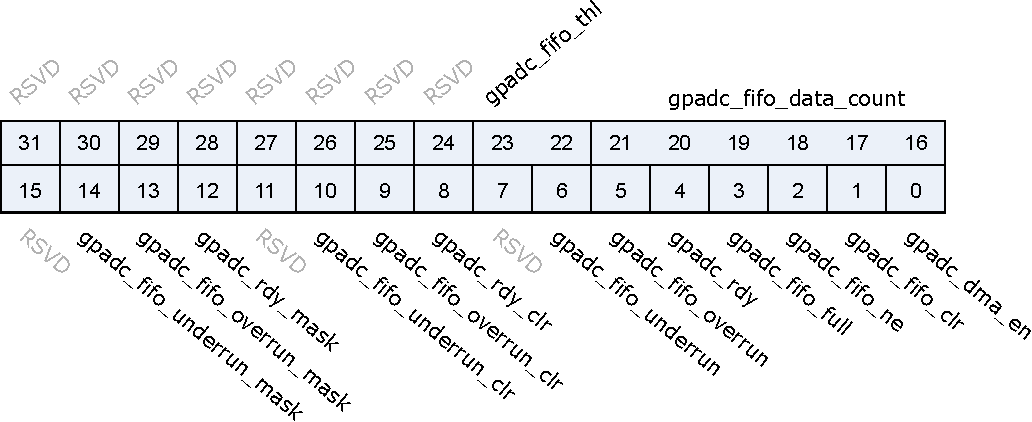
\includegraphics{gpip_gpadc_config.pdf}
\end{figure}

\regdes{31:24&RSVD& & & \\\hline
23:22&gpadc\_fifo\_thl&r/w&2'd0&fifo threshold \par 2'b00: 1 data  \par 2'b01: 4 data  \par 2'b10: 8 data \par 2'b11: 16 data
\\\hline
21:16&gpadc\_fifo\_data\_count&r&6'd0&fifo data number\\\hline
15&gpadc\_fifo\_rdy\_mask&r/w&1'b1&write 1 mask\\\hline
14&gpadc\_fifo\_underrun\_mask&r/w&1'b0&write 1 mask\\\hline
13&gpadc\_fifo\_overrun\_mask&r/w&1'b0&write 1 mask\\\hline
12&gpadc\_rdy\_mask&r/w&1'b0&write 1 mask\\\hline
11&RSVD& & & \\\hline
10&gpadc\_fifo\_underrun\_clr&w1c&1'b0&Write 1 to clear flag\\\hline
9&gpadc\_fifo\_overrun\_clr&w1c&1'b0&Write 1 to clear flag\\\hline
8&gpadc\_rdy\_clr&w1c&1'b0&Write 1 to clear flag\\\hline
7&gpadc\_fifo\_rdy&r&1'b0&FIFO ready interrupt flag\\\hline
6&gpadc\_fifo\_underrun&r&1'b0&FIFO underrun interrupt flag\\\hline
5&gpadc\_fifo\_overrun&r&1'b0&FIFO overrun interrupt flag\\\hline
4&gpadc\_rdy&r&1'b0&Conversion data ready interrupt flag\\\hline
3&gpadc\_fifo\_full&r&1'b0&FIFO full flag\\\hline
2&gpadc\_fifo\_ne&r&1'b0&FIFO not empty flag\\\hline
1&gpadc\_fifo\_clr&w1c&1'b0&FIFO clear signal\\\hline
0&gpadc\_dma\_en&r/w&1'b0&GPADC DMA enbale\\\hline

}
\subsection{gpadc\_dma\_rdata}
\label{gpip-gpadc-dma-rdata}
地址:0x40002004
 \begin{figure}[H]
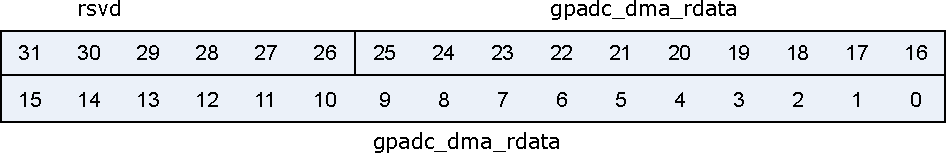
\includegraphics{gpip_gpadc_dma_rdata.pdf}
\end{figure}

\regdes{31:26&RSVD& & & \\\hline
25:0&gpadc\_dma\_rdata&r&26'd0&GPADC finial conversion result stored in the FIFO\\\hline

}
\subsection{gpdac\_config}
\label{gpip-gpdac-config}
地址:0x40002040
 \begin{figure}[H]
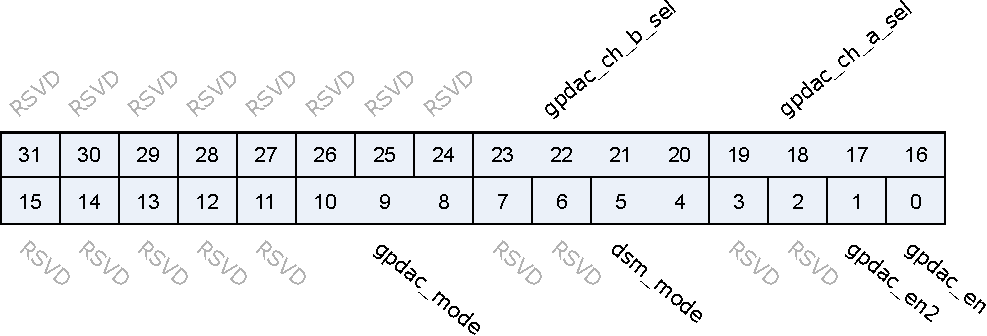
\includegraphics{gpip_gpdac_config.pdf}
\end{figure}

\regdes{31:24&RSVD& & & \\\hline
23:20&gpdac\_ch\_b\_sel&r/w&0&Channel B Source Select \par 0: Reg \par 1: DMA \par 2: DMA + Filter \par 3: Sin Gen \par 4: A (The same as channel A) \par 5: ~A (Inverse of channel A)
\\\hline
19:16&gpdac\_ch\_a\_sel&r/w&0&Channel A Source Select \par 0: Reg \par 1: DMA \par 2: DMA + Filter \par 3: Sin Gen
\\\hline
15:11&RSVD& & & \\\hline
10:8&gpdac\_mode&r/w&0&0:32k, 1:16k, 3:8k,  4:512k(for DMA only)\\\hline
7:6&RSVD& & & \\\hline
5:4&dsm\_mode&r/w&0&0:bypass, 1:dsm order=1, 2: dsm order=2\\\hline
3:2&RSVD& & & \\\hline
1&gpdac\_en2&r/w&0&GPDAC enable 2 (for B channel)\\\hline
0&gpdac\_en&r/w&0&GPDAC enable\\\hline

}
\subsection{gpdac\_dma\_config}
\label{gpip-gpdac-dma-config}
地址:0x40002044
 \begin{figure}[H]
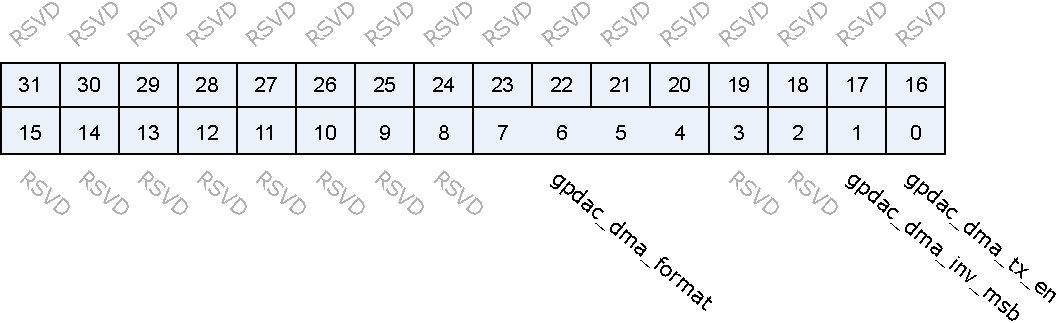
\includegraphics{gpip_gpdac_dma_config.pdf}
\end{figure}

\regdes{31:6&RSVD& & & \\\hline
5:4&gpdac\_dma\_format&r/w&0&DMA TX format (Data 12-bit) \par 0: {A0}, {A1}, {A2}… \par 1: {B0,A0}, {B1,A1}, {B2,A2}… \par 2: {A1,A0}, {A3,A2}, {A5,A4}… \par (Note: {20'h0,[11:0]} or {4'h0,[27:16],4'h0,[11:0]})
\\\hline
3:1&RSVD& & & \\\hline
0&gpdac\_dma\_tx\_en&r/w&0&GPDAC DMA TX enable\\\hline

}
\subsection{gpdac\_dma\_wdata}
\label{gpip-gpdac-dma-wdata}
地址:0x40002048
 \begin{figure}[H]
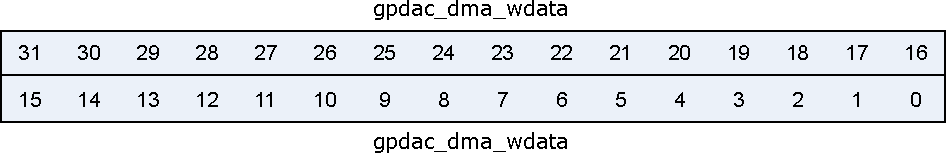
\includegraphics{gpip_gpdac_dma_wdata.pdf}
\end{figure}

\regdes{31:0&gpdac\_dma\_wdata&w&x&GPDAC DMA TX data\\\hline

}

\subsection{gpdac\_ctrl}
\label{glb-gpdac-ctrl}
地址:0x40000308
\begin{figure}[H]
	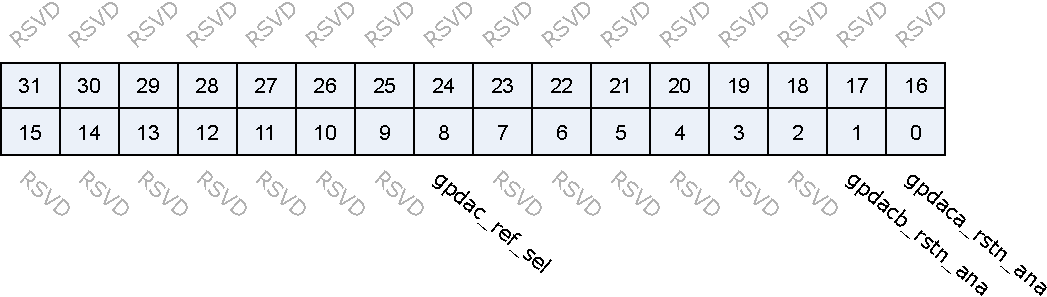
\includegraphics{glb_gpdac_ctrl.pdf}
\end{figure}

\regdes{31:9&RSVD& & & \\\hline
	8&gpdac\_ref\_sel&r/w&1'h0&Reference select \par 1'h0 Internal reference \par 1'h1 External reference
	\\\hline
	7:2&RSVD& & & \\\hline
	1&gpdacb\_rstn\_ana&r/w&1'h1&Soft reset for DAC channel B, active low\\\hline
	0&gpdaca\_rstn\_ana&r/w&1'h1&Soft reset for DAC channel A, active low\\\hline
	
}
\subsection{gpdac\_actrl}
\label{glb-gpdac-actrl}
地址:0x4000030c
\begin{figure}[H]
	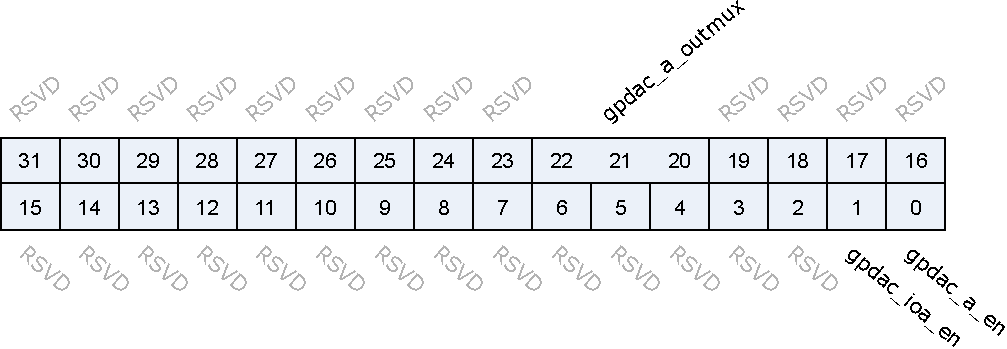
\includegraphics{glb_gpdac_actrl.pdf}
\end{figure}

\regdes{31:23&RSVD& & & \\\hline
	22:20&gpdac\_a\_outmux&r/w&3'h0&\\\hline
	19:18&gpdac\_a\_rng&r/w&2'h3&Output voltage range control with internal/external reference\\\hline
	17:2&RSVD& & & \\\hline
	1&gpdac\_ioa\_en&r/w&1'h0&Channel A conversion output to pad enable \par 1'h0 Disable channel A conversion result to GPIO \par 1'h1 Enable channel A conversion result to GPIO
	\\\hline
	0&gpdac\_a\_en&r/w&1'h0&Channel A enable/disable signal \par 1'h0 Disable channel A conversion. \par 1'h1 Enable channel A conversion
	\\\hline
	
}
\subsection{gpdac\_bctrl}
\label{glb-gpdac-bctrl}
地址:0x40000310
\begin{figure}[H]
	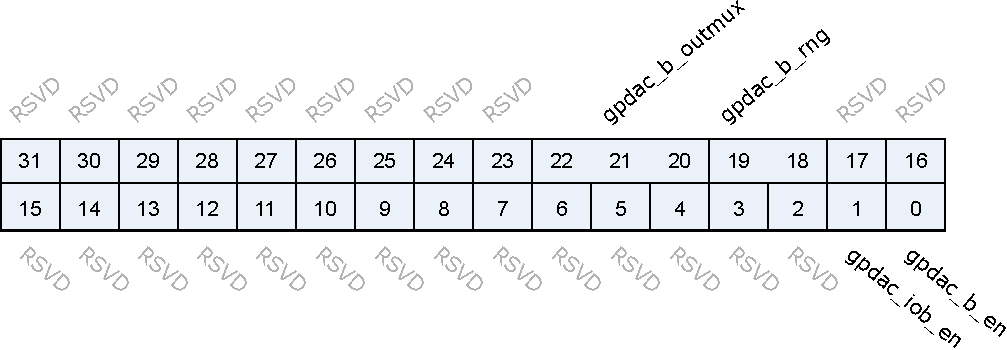
\includegraphics{glb_gpdac_bctrl.pdf}
\end{figure}

\regdes{31:23&RSVD& & & \\\hline
	22:20&gpdac\_b\_outmux&r/w&3'h0&\\\hline
	19:18&gpdac\_b\_rng&r/w&2'h3&\\\hline
	17:2&RSVD& & & \\\hline
	1&gpdac\_iob\_en&r/w&1'h0&channel B conversion output to pad enable \par 1'h0 Disable channel B conversion result to GPIO \par 1'h1 Enable channel B conversion result to GPIO
	\\\hline
	0&gpdac\_b\_en&r/w&1'h0&channel B enable/disable signal \par 1'h0 Disable channel B conversion. \par 1'h1 Enable channel B conversion
	\\\hline
	
}
\subsection{gpdac\_ctrl}
\label{glb-gpdac-ctrl}
Address:0x40000308
\begin{figure}[H]
	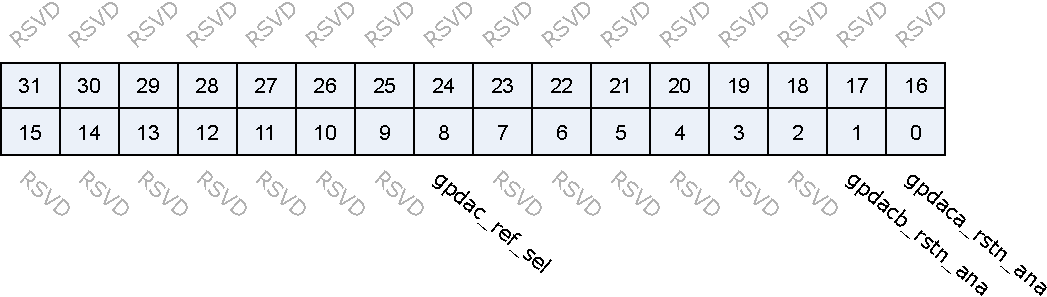
\includegraphics{glb_gpdac_ctrl.pdf}
\end{figure}

\regdes{31:9&RSVD& & & \\\hline
	8&gpdac\_ref\_sel&r/w&1'h0&Reference select \par 1'h0 Internal reference \par 1'h1 External reference
	\\\hline
	7:2&RSVD& & & \\\hline
	1&gpdacb\_rstn\_ana&r/w&1'h1&Soft reset for DAC channel B, active low\\\hline
	0&gpdaca\_rstn\_ana&r/w&1'h1&Soft reset for DAC channel A, active low\\\hline
	
}
\subsection{gpdac\_actrl}
\label{glb-gpdac-actrl}
Address:0x4000030c
\begin{figure}[H]
	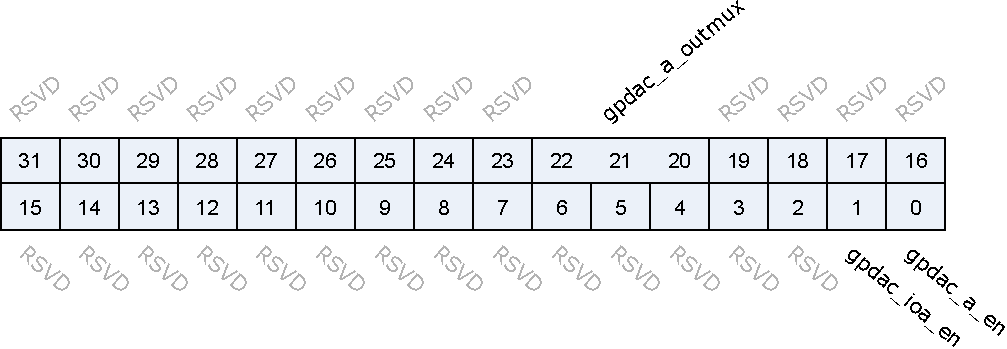
\includegraphics{glb_gpdac_actrl.pdf}
\end{figure}

\regdes{31:23&RSVD& & & \\\hline
	22:20&gpdac\_a\_outmux&r/w&3'h0&\\\hline
	19:18&gpdac\_a\_rng&r/w&2'h3&Output voltage range control with internal/external reference\\\hline
	17:2&RSVD& & & \\\hline
	1&gpdac\_ioa\_en&r/w&1'h0&Channel A conversion output to pad enable \par 1'h0 Disable channel A conversion result to GPIO \par 1'h1 Enable channel A conversion result to GPIO
	\\\hline
	0&gpdac\_a\_en&r/w&1'h0&Channel A enable/disable signal \par 1'h0 Disable channel A conversion. \par 1'h1 Enable channel A conversion
	\\\hline
	
}
\subsection{gpdac\_bctrl}
\label{glb-gpdac-bctrl}
Address:0x40000310
\begin{figure}[H]
	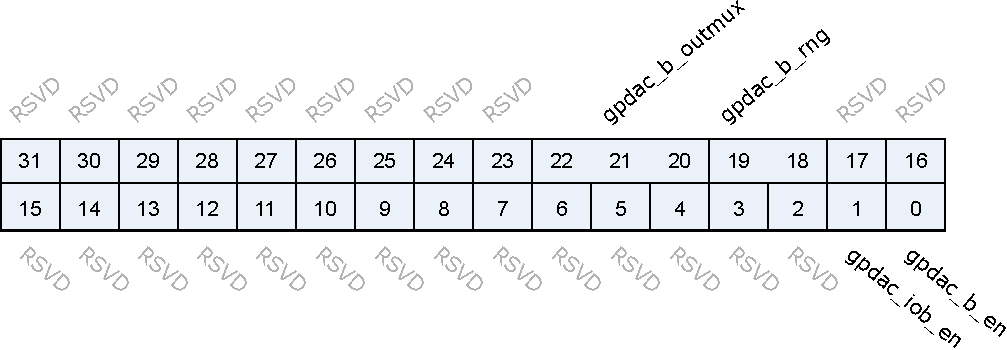
\includegraphics{glb_gpdac_bctrl.pdf}
\end{figure}

\regdes{31:23&RSVD& & & \\\hline
	22:20&gpdac\_b\_outmux&r/w&3'h0&\\\hline
	19:18&gpdac\_b\_rng&r/w&2'h3&\\\hline
	17:2&RSVD& & & \\\hline
	1&gpdac\_iob\_en&r/w&1'h0&channel B conversion output to pad enable \par 1'h0 Disable channel B conversion result to GPIO \par 1'h1 Enable channel B conversion result to GPIO
	\\\hline
	0&gpdac\_b\_en&r/w&1'h0&channel B enable/disable signal \par 1'h0 Disable channel B conversion. \par 1'h1 Enable channel B conversion
	\\\hline
	
}
